\documentclass[pdf]{beamer}
\usepackage{listings}
\usepackage{color}

\definecolor{dkgreen}{rgb}{0,0.6,0}
\definecolor{gray}{rgb}{0.5,0.5,0.5}
\definecolor{mauve}{rgb}{0.58,0,0.82}

\lstset{frame=none,
language=C,
columns=flexible,
numberstyle=\tiny\color{gray},
keywordstyle=\color{blue},
commentstyle=\color{dkgreen},
stringstyle=\color{mauve},
breaklines=true,
breakatwhitespace=true,
tabsize=4,
showstringspaces=false,
basicstyle=\ttfamily
}
\usepackage{parskip}
\usepackage{graphicx}
\graphicspath{{../images/}}

\mode<presentation>
{
	\usetheme{default}      % or try Darmstadt, Madrid, Warsaw, ...
	\usecolortheme{default} % or try albatross, beaver, crane, ...
	\usefonttheme{default}  % or try serif, structurebold, ...
	\setbeamertemplate{navigation symbols}{}
	\setbeamertemplate{caption}[numbered]
}

\begin{document}
\title{Intel Cloud Orchestration Networking Design and Goals}
\author{Matthew Johnson, Cody Malick, and Garrett Smith}
\date{7 December, 2016}

\maketitle
\begin{frame}
	\frametitle{Table of Contents}
	\tableofcontents
\end{frame}

\begin{frame}
	\frametitle{Team Cloud Orchestra}
	\section{Introduction}
	Our team is implementing a software defined network based on Open
	vSwitch for a cloud orchestration technology called Ciao.

	Our client is Rob Nesius, Engineering Manager at Intel Corporation.
\end{frame}

\begin{frame}
	\frametitle{Scope}
	\section{Scope}
	What is a cloud?
	\begin{figure}[H]
		\caption{The Cloud - Randall Munroe~\cite{xkcd908}}
		\begin{center}
			\makebox[\textwidth]{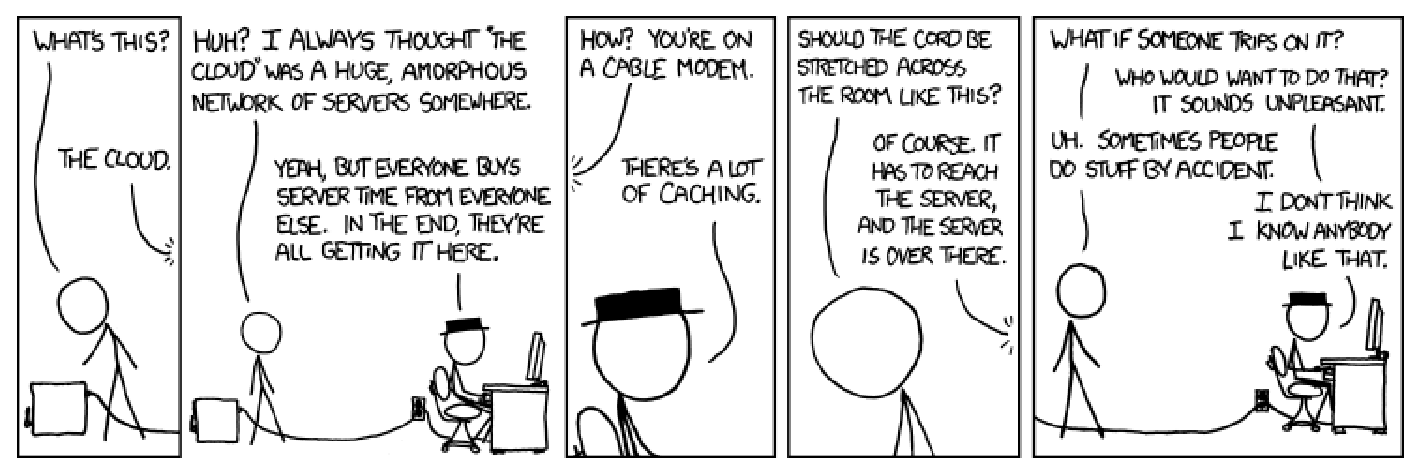
\includegraphics[width=\textwidth]{xkcd.eps}}
		\end{center}
	\end{figure}

	"A huge, amorphous network of servers somewhere"

\end{frame}

\begin{frame}
	\frametitle{Scope}
	The network connecting the nodes must be controlled. In our case, this
	is achieved by the Cloud Integrated Advanced Orchestrator, or Ciao.

	Ciao provides an easy to deploy, secure, scalable cloud orchestration
	system which handles virtual machines, containers, and bare metal apps
	agnostically as generic workloads~\cite{ciao}.
\end{frame}

\begin{frame}
	\frametitle{Scope}
	The servers, or nodes, in these clouds need to talk to each other, hence
	the need for a network solution.

	Ciao uses a software defined network to allow different compute nodes to
	communicate with each other.

	Software defined networking is a software abstraction of physical
	networking solutions, allowing for ``a more scalable and centralized
	network control architecture''~\cite{goransson}.
\end{frame}

\begin{frame}
	\frametitle{Project Goals}
	\framesubtitle{Goal One}
	\section{Project Goals}
	Switch Ciao Generic Routing Encapsulation (GRE) tunnel implementation to
	use Open vSwitch-created GRE tunnels.

	\begin{description}[style=nextline]
		\item[Generic Routing Encapsulation (GRE)]
			GRE encapsulates an arbitrary network layer protocol so
			it can be sent over arbitrary network layer
			protocol~\cite{rfc1701}.
		\item[Open vSwitch (OVS)]
			Open vSwitch is a ``multilayer virtual switch\ldots
			designed to enable massive network automation through
			programmatic extension''~\cite{ovs}.
	\end{description}
\end{frame}

\begin{frame}
	\frametitle{Project Goals}
	\framesubtitle{Goal Two}
\end{frame}

\begin{frame}
	\frametitle{Project Goals}
	\framesubtitle{Goal Three (optional)}
\end{frame}

\begin{frame}
	\frametitle{Project Design}
	\section{Open vSwitch Database Management Protocol}
	Open vSwitch uses a database to manage configuration while running.
	The configuration can be updated on the fly by accessing its management
	protocol using the Open vSwitch Database Management Protocol, defined
	in RFC 7047\cite{rfc7047}
\end{frame}

\begin{frame}[fragile]
	\frametitle{Libovsdb}
	Libovsdb is an open source library that provides a Go programming
	language wrapper around the OVS Database Management Protocol. Here is
	an example:\cite{gosample} \\

\begin{lstlisting}[caption=Example insert operation using libovsdb]
	// simple insert operation
	insertOp := libovsdb.Operation{
	    Op:	  "insert",
	    Table:	  "Bridge",
	    Row:	  bridge,
	    UUIDName: namedUUID,
	}

\end{lstlisting}
\end{frame}
\begin{frame}
	\frametitle{nvGRE and VxLAN}
	Two alternative tunneling protocols to replace GRE, the current
	protocol used by Ciao.\\
	nvGRE: Network virtualization standard created in tandem by HP, Dell,
	and Intel
	VxLAN: Network virtualization standard created in tandem by Cisco,
	VMware, Citrix, and Redhat

	Overall performance and overhead are similar on paper, will require
	testing to see which is the best fit for our implementation
\end{frame}
\begin{frame}
	\frametitle{Stumbling Blocks}
	Stumbling blocks go here
\end{frame}

\begin{frame}
\end{frame}
\begin{frame}
	\frametitle{References}
		\bibliographystyle{IEEEtran}
		\bibliography{pres}
	\end{frame}
\end{document}
